\section{Introduction}

\begin{figure}[t]
\centering
\includegraphics[width=0.45\textwidth]{figures/taxonomylabels}
 \caption{An example of geographical taxonomy with Dewey codes}
\label{fig:toytaxonomyexample}
\end{figure}


A string join, which finds all equivalent string pairs between two input collections, is an essential operation in many applications, such as  data integration \cite{conf/sigmod/Sarawagi04}, data cleansing \cite{conf/vldb/ArasuGK06,journals/www/LiJM06} and information extraction \cite{books/Winkler99}. In practice, the same object/entity may have different representations  due to a variety of reasons such as misspellings and  formatting variations. Hence, it is important to support approximate string joins to reconcile different
representations of the same entity. A large number of  similarity functions such as Levenshtein distance~\cite{conf/sigmod/WangLF12},
Hamming distance~\cite{conf/spire/Kondrak05}, Overlapping coefficient~\cite{conf/icde/ChaudhuriGK06}, Cosine
metric~\cite{journals/ipm/SaltonB88}, Jaccard
Coefficient~\cite{conf/icde/ChaudhuriGK06,conf/icde/LiLL08}, JaccT \cite{conf/icde/ArasuCK08} and Synonym-based similarity \cite{conf/sigmod/LuLWLW13} have been proposed in the literature. It is well known
that no single similarity function is universally applicable
across all domains and scenarios~\cite{conf/ijcai/CohenRF03}.

In this paper, we investigate a problem to exploit taxonomies with string similarity joins. In principle, a taxonomy presents a general purpose strategy to improve the accuracy of string joins by enriching data with semantics-based knowledge. Taxonomies are sets of IS-A hierarchies, which identify the relations between different concepts. The IS-A relationship
is a transitive closure of the concept-instance relationship.
For example, if ``\textsf{kitten}'' is an instance of ``\textsf{cat}'', and
``\textsf{cat}'' is an instance of ``\textsf{pet}'', then ``\textsf{kitten}'' is an instance
of ``\textsf{pet}''. If we treat each term as a node, and create
for each (\textsf{concept}, \textsf{instance}) pair, an edge from the concept
to the instance, then we can think of a taxonomy as a tree or forest. For any node that represents a term,
the IS-A relation could be any descendant of it in the tree. Figure
\ref{fig:toytaxonomyexample} shows a toy example of a geographical taxonomy tree.

Based on the taxonomy,  the similarity of two strings can be measured in a \textit{semantic} way. For example, consider two strings ``\textsf{Cupertino}'' and ``\textsf{California}''. Based on a syntactic-level similarity function, such as $n$-gram Jaccard similarity~\cite{conf/icde/ChaudhuriGK06,conf/icde/LiLL08}, the similarity of two strings is zero. But note that ``\textsf{Cupertino}'' is a city in ``\textsf{California}''. If we use the geological taxonomy tree in Figure \ref{fig:toytaxonomyexample} to calculate the longest common prefixes (LCP) between these two strings, then LCP(``\textsf{Cupertino}'', ``\textsf{California}'')= 4, which indicates the closeness of two concepts. In contrast, consider another two strings
 ``\textsf{Cupertino}'' and ``\textsf{Seoul}''. Note that LCP(``\textsf{Cupertino}'', ``\textsf{Seoul}'')=1$<$4, because ``\textsf{Cupertino}'' and ``\textsf{Seoul}'' locate in two different continents as indicated in the taxonomy tree.


\begin{figure}[t]
\centering
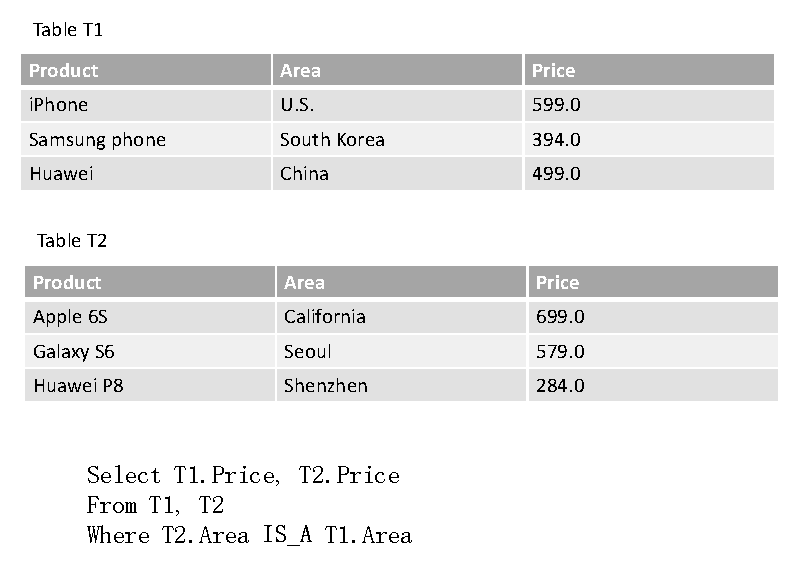
\includegraphics[width=0.45\textwidth]{figures/productexample}
 \caption{Two tables about cellphones for data integration}
\label{fig:twotables}
\end{figure}

We give several applications to shed light on the importance of the string similarity matching with taxonomies on data management.

\begin{itemize}
  \item \textbf{Data Integration} ~ Data integration involves combining data residing in different sources. Taxonomies are quite useful to  integrate the objects with IS-A relations. For example, consider two tables in Figure \ref{fig:twotables}. In order to correctly join the records between two tables, one needs to know hat ``\textsf{Apple 6S is a model of iPhone}'' and ``\textsf{California is a state in U.S.}'', and etc. A join mechanism that can utilize such taxonomy knowledge may help users to discover more relevant records and thus to improve the effectiveness of data integration.

       \item \textbf{Data cleansing}~  Data cleansing is the process of detecting and correcting (or removing) corrupt or inaccurate records from a table or database. For example, two records about ``\textsf{Sumsung cellphone}'' and ``\textsf{Glaxy S6}'' may contain the duplicate or inconsistent information, because ``\textsf{Glaxy S6}'' IS-A model of ``\textsf{Sumsung cellphones}''. In those scenarios, a string join algorithm with taxonomies can enhance the quality of data cleansing by identifying more relevant records.

  \item \textbf{Information extraction}~  Information extraction (IE) is the task of automatically extracting structured information from unstructured and/or semi-structured documents. For example, a typical task is to ``\textit{find all geological entities in U.S.}'' in a document. A new similarity search tool based on a geological taxonomy can handle term variation and thus extract more locations of interests.
\end{itemize}

% \item \textbf{Data mining} ~ Term classification and term clustering are two important tasks in data mining. A new similarity measure that can find the IS-A relations between terms may boost the accuracies of term classification and clustering \cite{journals/dke/CaglieroG13}.



  %\item \textbf{Information extraction} Find all geological entity in U.S. Then a new similarity measure based on a geological taxonomy can handle term variation and discover more location of interests





%  Conceptually, there are two cases of string joins: \textit{exact-joins} and \textit{approximate-joins}. Exact joins mean that two matching strings are exactly the same, while approximate joins tolerate certain difference between two strings and the similarity between two strings is measured by a similarity function, such as  Levenshtein distance~\cite{conf/sigmod/WangLF12},
%Hamming distance~\cite{conf/spire/Kondrak05}, Episode
%distance~\cite{conf/ijcai/CohenRF03}, Cosine
%metric~\cite{journals/ipm/SaltonB88}, Jaccard
%Coefficient~\cite{conf/icde/ChaudhuriGK06,conf/icde/LiLL08}, and Dice
%similarity~\cite{conf/www/BayardoMS07}.

\subsection{Overview and contributions}

In this paper, we assume that we already have complete
information of these IS-A relations, i.e. \textit{taxonomy}, and we will focus on how
to effectively utilize these information to  perform efficient string similarity joins. In particular, we first explore a special yet fundamental case: any string in a collection matches only one node in taxonomy trees, such as  ``\textsf{California}''  and ``\textsf{Michigan}'' in Figure \ref{fig:toytaxonomyexample}.   In this case, we present an LCP-based similarity function and  develop two families of join algorithms. The first is performed on the sorted lists of input data, while the second utilizes the compact tries structures. We analyze both algorithms and show that the second is optimal among all sequential algorithms that read the entire input, and has the worst-case complexity linear in the sum of input and output sizes.

 %We study the above two problems in two scenarios:  In the first special yet common  scenario, each string in a collection matches only one node in a taxonomy tree, like ``\textsf{California}''  and ``\textsf{iPhone}'' in the previous examples; and in the second scenario, one string can match multiple nodes in a taxonomy.

%For example, the (Guangdong, Shenzhen) is a (concept, instance) pair and (Shenzhen, China) has the IS-A relation, as Shenzhen is a city in China.
% Given two collections of strings $S$ and $T$, and a threshold $\theta$, we then study how to find all string pairs ($s, t$) $\in S \times T$ such that $f(s,t) > \theta$.




 %the first challenge is to devise new similarity functions. Although there is a wealth of string similarity functions \cite{conf/spire/Kondrak05,conf/ijcai/CohenRF03,journals/ipm/SaltonB88,conf/icde/ChaudhuriGK06,conf/icde/LiLL08}, most of them focus on only the syntactical-level of words, except for recent works  \cite{conf/icde/ArasuCK08,conf/sigmod/LuLWLW13} which have studied the similarity functions based on synonyms. But taxonomy is quite different from synonym in that taxonomy represents a tree-like structure, while synonym deals with binary relations between words. Meanwhile, we note that other existing works in the domains of natural language processing \cite{journals/jair/Resnik99} and bioinformatics \cite{journals/jbi/McInnesP13} also studied similarity measures with taxonomy. Their methods, while pioneering and interesting, focus on the textual documents and are not directly applicable to string joins in tables.



Then we turn to a generalized case, when one string matches multiple nodes in taxonomy trees.  For example, consider two strings: ``\textsf{Riverside California}'' and ``\textsf{Cupertino US}'', either of which matches two nodes in  Figure \ref{fig:toytaxonomyexample}. In this scenario, we extend the previous LCP-based function by borrowing the maximum nodes matching in a bipartite graph. We prove that our new similarity measurement satisfies three attractive properties, called the three C's. that naturedly captures the attributes of the similarity with taxonomies: \textit{Constructive}, \textit{Compatible} and \textit{Consistent}. We extend the Hungarian algorithm \cite{journals/JSIAM/Munkres57} to compute this new scoring function.


%(1) \textit{Constructive}:  taxonomies are always constructive to the similarity. In other words, the utilization of taxonomy cannot decrease the similarity of two strings; (2) \textit{Compatible}: the similarity is compatible with the insertion of taxonomy nodes. That is, the insertion of new nodes in a taxonomy tree cannot decrease the similarity; Finally, (3) \textit{Consistent}:  the similarity of two string lie in
%the range [\textit{min}, \textit{max}], where \textit{min} and \textit{max} denotes the min and max similarity for any two single tokens in two strings respectively.

% Before presenting our new function, we describe three properties, called the three C's:  \textit{Constructive}, \textit{Compatible} and \textit{Consistent},  that capture the attributes of the similarity with taxonomy.

%(See Section 2 for more explanations of why the existing similarity functions are not applicable for taxonomy).


%Given the newly similarity functions, it is imperative to study efficient similarity join algorithms. The brute-force algorithm that enumerates every string pair and checks whether the two strings in the pair are similar is rather expensive.

To realize the efficient string joins in the generalized case,
unfortunately, the join algorithm based on the previous special case
cannot work again. Therefore, we develop a new algorithm to adopt a
filter-verification framework \cite{conf/cpm/SutinenT96,conf/sigmod/LuLWLW13}, which includes two steps: (1) Filter step: devising effective filtering algorithms to prune large numbers of dissimilar pairs and generating a set of candidate pairs; and (2) Verification step: verifying each candidate pair by computing
the real similarity and outputting the final results. Since the verification step is a time-consuming step,  filtering algorithms play an important role in this framework.  The existing filtering techniques include count filtering \cite{conf/vldb/GravanoIJKMS01}, length filtering \cite{conf/vldb/ArasuGK06}, position
filtering \cite{conf/esa/SutinenT95} and prefix filtering \cite{conf/sigmod/WangLF12}, etc. In this paper, we extend count filters by proposing a new filter called Semantics-Similar filters (SS-filters). The existing count filters assume that two strings are similar only if they share enough number of common tokens. Unfortunately, this assumption does not hold in our setting. For example, consider two strings ``\textsf{Cupertino, US}'' and ``\textsf{California}'', which share no common tokens, but  they are ``similar'' in the sense that both refer to the same country and state.   Our new observation is that \textit{two strings are similar if they share enough number of ``Semantics-Similar'' (not the same) tokens}. Recall the above example, where ``\textsf{California}'' is semantics-similar to both ``\textsf{Cupertino}'' and ``\textsf{US}'', but
``\textsf{California}'' is not the same as ``\textsf{Cupertino}'' and ``\textsf{US}''.

%Therefore, in the problem setting of string joins with taxonomies, two strings are similar if they share enough numbers of semantically similar tokens.




  It turns out that SS-filters have two intertwined thresholds: the similarity threshold $\theta$ between tokens  and the number of similar token pairs $\tau$, as $\theta$ grows and shrinks, $\tau$ must be  adjusted
in such a way that all similar strings should be conserved. Consequently, with varied  $\theta$ and $\tau$, there exists a set of different SS-filters. Note that there is a tradeoff between filtering time and verification time with SS-filters. In particular, if we employ more SS-filters to prune away more string pairs, then  it could reduce verification time but increase filtering time. On the other hand, if we reduce the number of filters employed, it could decrease filtering time, but causing more time for verification. Therefore,  an optimization problem is to select a subset of SS-filters to aim at minimizing the total running time. In this paper, we prove the NP-hardness of this problem by reduction from classic set-cover problems, and propose an efficient greedy algorithm.


The challenge in this greedy  algorithm is that we need to quickly
compute the filtering effectiveness of SS-filters with varied
parameters of $\theta$ and $\tau$. Note that it is unrealistic to know
the accurate number of string pairs which a given SS-filter can prune,
since it would lead to an actual filtering, which is
prohibitively expensive. Therefore, in
this paper, our technical contribution is to develop a 
sampling algorithm to estimate the filtering power
of SS-filters. The salient feature of this sampling is that, instead of fixing the size of sampled strings, according to the hardness of join instances, it initially specifies confidence and time bounds, and  uses the sampled data adaptively until the confidences are achieved or the allocated time is used. The advantage of this algorithm is that it can quickly estimate the results  with a small set of samples.  We apply results from the theories of order statistics \cite{journals/jcss/Cohen97} and hypergeometric distributions \cite{conf/sigmod/BeyerHRSG07} to show that this adaptive sampling algorithm is unbiased. We also derive the probabilistic error bounds, which can be used to determine appropriate sample sizes.
 
% Our estimation algorithm proposes the use of KMV synopsis, extending an idea in \cite{conf/sigmod/BeyerHRSG07} to handle $\tau$-occurrence, our extension involves adding an inverted lists to the basic synopsis, to find the $\tau$-occurrence. Using a probabilistic model of hashing, we apply results from the theory of order statistics to show that our proposed estimator is unbiased and has small relative error.   We present an estimation algorithm that estimate the power of an SS-filter, high confidence estimates with small relative error. For any fixed $\epsilon > 0$ and $ \delta \in $ (0,1], our estimates for $\tau$-occurrence and filter join are such that with probability at least 1-$\delta$, the respective relative error ($\frac{|T-\hat{T}|}{|T|}$) is at most $\epsilon$.

 %
% Our method carries both theoretical and empirical benefits. In
%theory, we can prove that, with high probability 1-$\delta$,
%our estimation accurately return the upper and lower bounds of the filtering power of a similarity filter, and its space
%and time complexities are logarithmic in the cardinality of input size.
%In practice, the experiments show that our estimation technique
%accurately predicts the quality of different similarity filters and its running time is negligible compared to that of the actual filtering phase (accounting for only 1\% of the total join time).




\smallskip

Finally, we perform a comprehensive set of experiments on three data sets to demonstrate the superior efficiency of our algorithms. The results show that our algorithm can utilize taxonomies to improve the effectiveness of string joins  and  scale very well with important parameters like data size and taxonomy size. The adaptive sampling algorithm offers good results and is efficient to select high-quality SS-filters (which samples only 1-2\% data to select high-quality filters in most cases), which motivates its application in practice.


\smallskip

The rest of this paper is organized as follows. Section 1.2 presents the related work. Section 2
provides the necessary definitions, formulates . Section
3 includes our algorithm for exact joins with taxonomy. In Section 4, we study
the approximate string join, proposing our solution, analyzing its approximation
ratio, and presenting our similarity join algorithms.
Our experiments are presented in Section 5. Finally,
Section 6 concludes with a discussion about future work.

\subsection{Related work}

A string similarity join an essential operation in
 many applications, such as data integration, data cleansing and information extraction.  A comparison of many string similarity functions is performed in \cite{conf/ijcai/CohenRF03}. There has been much recent work and progress on efficient string similarity joins  \cite{conf/sigmod/LuLWLW13,conf/icde/ArasuCK08,conf/cpm/BarbayGMR06,conf/vldb/ArvindSR09} and most of them follow the filter-and-verification framework.  Add more related works on filtering!!
 
 
 
 Taxonomy is the practice and science of classification.  A taxonomy could be constructed manually through experts and community efforts, as in WordNet \cite{books/fellbaum1998wordnet} and Freebase \cite{conf/aaai/BollackerCT07}, or automatic taxonomy construction, for example, in WikiTaxonomy \cite{conf/ecai/PonzettoS08} and YAGO \cite{conf/cidr/MahdisoltaniBS15}.

\smallskip


String semantic similarity \cite{conf/cikm/SayedHZ07,conf/cl/WuP94,journals/jair/Resnik99}, which has been studied in some fields as natural language processing (NLP) and artificial intelligence (AI), is defined over a set of documents or terms. The semantic relatedness (such as, latent semantic analysis \cite{conf/cscl/LandauerD02},  pointwise mutual information \cite{conf/pkdd/Schneider05} )  between units of language (e.g., words, sentences) can be estimated using statistical means such as a vector space model to correlate words and textual contexts from a suitable text corpus. In this paper, we study string semantics from the views of data management by proposing efficient join algorithms with taxonomy knowledge.

%The existing semantic functions can be classified to single-word level and multiple-words level. For the single-word level, computationally, semantic similarity can be estimated by defining a topological similarity, by using ontologies to define the distance between terms/concepts. For example, a naive metric for the comparison of concepts ordered in a partially ordered set and represented as nodes of a taxonomy tree, would be the shortest-path linking the two concept nodes.  For the multiple-words level, it can be grouped into two categories:  (1) those that view a text as a combination of words and calculate the similarity of two texts by aggregating the similarities of word pairs across the two texts, and (2) those that model a text as a whole and calculate the similarity of two texts by comparing the two models obtained. Approaches in the first category search for pairs of words across the two texts that maximize similarity and compute the overall similarity by aggregating individual similarity values, either by exploiting large text corpora [96], [26], [97], [98] and [99], or thesauri [100], sometimes also taking into account the word order in the text [101]. In this paper, we propose a new similarity function following the first line. The second category usually involves transforming texts into vectors and computing the similarity of texts by comparing their corresponding vectors. Vector space models [21] are an early example of this category, an idea borrowed from Information Retrieval. The initial models mainly focused on the representation of larger pieces of text, such as documents, where a text is modeled on the basis of the frequency statistics of the words it contains. Such models, however, suffer from sparseness and cannot capture similarities between short text pairs that use different wordings. A more suitable vector representation for shorter textual items is one that is based on semantic composition, and that seeks to model a text by combining the representations of its individual words [102]. A thorough study and comparison of different compositionality strategies is provided in [103], [104] and [105]. Recently, an approach mixing distributional information and explicit knowledge has been successfully applied to cross-lingual document retrieval and categorization [106].




 

%Finally, in recent years, there is the emergence of various efforts to enhance the effectiveness of string similarity joins by using synonyms \cite{conf/sigmod/LuLWLW13,conf/icde/ArasuCK08,conf/cpm/BarbayGMR06,conf/vldb/ArvindSR09}.
%Given two collections of strings,  synonym-based similarity functions can utilize the available synonyms to find string pairs which are semantically similar. While those methods improve the effectiveness of string joins, a synonym dictionary does not contain information such as `\textsf{`Apple 6 Plus is a new model of iPhone}''. Still, term pairs ``\textsf{Apple 6 Plus}'' and ``\textsf{iPhone}''  have strong semantic correlations. This paper pushes the research frontier forward by studying the joins with another common type of semantics: taxonomies.



